\documentclass[a4paper]{article}
\usepackage{import}
\usepackage{graphicx}
\usepackage{float}
\usepackage{pgfplots}
\usepackage{listings}
\usepackage{enumitem}
\usepackage{textcomp}
\usepackage{tikz}
\usetikzlibrary{decorations.pathreplacing} % for angle arc
\usetikzlibrary{angles, quotes, calc, positioning, trees} % for drawing angles
\pgfplotsset{compat=1.18,width=10cm}
\usepackage{tikz-cd}
\usepackage{booktabs}
\usepackage{cancel}
\usepackage{amsmath}
\usepackage{minted}
\usepackage{csquotes}
\usepackage{gensymb}
\usepackage{forest}
\usepackage{amsthm}
\usepackage{amssymb}
\usepackage{fontawesome} 
\usepackage{varwidth}
\usepackage{pgfplots}
\usepackage{lipsum}
\usepackage{mdframed} 
\usepackage{color}   
\usepackage{hyperref}
\newmdtheoremenv{theo}{Theorem}
\usepackage{mathtools}
\DeclarePairedDelimiter\ceil{\lceil}{\rceil}
\DeclarePairedDelimiter\floor{\lfloor}{\rfloor}

\hypersetup{
    colorlinks=true, %set true if you want colored links
    linktoc=all,     %set to all if you want both sections and subsections linked
    linkcolor=black,  %choose some color if you want links to stand out
}

% Define theorem styles
\newtheorem{theorem}{Theorem}[section]    % Theorems numbered within sections
\newtheorem{lemma}[theorem]{Lemma}        % Lemmas use the same counter as theorems
\newtheorem{corollary}[theorem]{Corollary} % Corollaries use the same counter as theorems
\newtheorem{proposition}[theorem]{Proposition} % Proposition uses the same counter
\newtheorem{property}[theorem]{Property}
\theoremstyle{definition}
\newtheorem{definition}[theorem]{Definition} % Now uses the same counter as theorems


% Remark-style theorem
\theoremstyle{remark}
\newtheorem{remark}[theorem]{Remark}

% Boxed environment for theorems
\newmdenv[
  linewidth=0.8pt,
  roundcorner=5pt,
  linecolor=black,
  backgroundcolor=white!5,
  skipabove=\baselineskip,
  skipbelow=\baselineskip,
  innerleftmargin=10pt,
  innerrightmargin=10pt,
  innertopmargin=5pt,
  innerbottommargin=5pt
]{thmbox}

% Custom proof environment (also boxed)
\renewenvironment{proof}[1][Proof]{%
  \begin{mdframed}[linewidth=0.8pt, roundcorner=5pt, linecolor=black, skipabove=\baselineskip, skipbelow=\baselineskip, innertopmargin=5pt, innerbottommargin=5pt]%
  \noindent\textbf{#1. }%
}{%
  \end{mdframed}%
}

% Redefine theorem environments to use thmbox
\let\oldtheorem\theorem
\renewenvironment{theorem}{\begin{thmbox}\begin{oldtheorem}}{\end{oldtheorem}\end{thmbox}}

\let\oldlemma\lemma
\renewenvironment{lemma}{\begin{thmbox}\begin{oldlemma}}{\end{oldlemma}\end{thmbox}}

\let\oldcorollary\corollary
\renewenvironment{corollary}{\begin{thmbox}\begin{oldcorollary}}{\end{oldcorollary}\end{thmbox}}

\let\oldproposition\proposition
\renewenvironment{proposition}{\begin{thmbox}\begin{oldproposition}}{\end{oldproposition}\end{thmbox}}

\let\oldproperty\property
  \renewenvironment{property}{\begin{oldproperty}}{\end{oldproperty}}


% Reference shortcuts
\newcommand{\thmref}[1]{Theorem~\ref{#1}}
\newcommand{\lemref}[1]{Lemma~\ref{#1}}
\newcommand{\corref}[1]{Corollary~\ref{#1}}
\newcommand{\propref}[1]{Property~\ref{#1}} 

% To customize QED symbol
\renewcommand{\qedsymbol}{$\blacksquare$}

\usetikzlibrary{decorations.pathreplacing} % for angle arc
\usetikzlibrary{angles, quotes, calc} % for drawing angles

\usepackage{color}   %May be necessary if you want to color links
\usepackage{hyperref}
\hypersetup{
    colorlinks=true, %set true if you want colored links
    linktoc=all,     %set to all if you want both sections and subsections linked
    linkcolor=black,  %choose some color if you want links to stand out
}

\usepackage{xcolor}
\usepackage[most]{tcolorbox}


% Define a custom tcolorbox environment for examples
\newtcolorbox{examplebox}[2][]{
  colback=blue!5!white,
  colframe=blue!30!black,
  title=#2,
  boxrule=0mm,
  fonttitle=\bfseries,
  width=\textwidth,
  breakable,
  #1
}

\newtcolorbox{definizione}[2] {
  colback=green!5!white,
  colframe=green!30!black,
  title=#2,
  boxrule=0mm,
  fonttitle=\bfseries,
  width=\textwidth,
  breakable,
  #1
}

\definecolor{codegreen}{rgb}{0,0.6,0}
\definecolor{codegray}{rgb}{0.5,0.5,0.5}
\definecolor{codepurple}{rgb}{0.58,0,0.82}
\definecolor{backcolour}{rgb}{0.95,0.95,0.92}

\lstdefinestyle{mystyle}{
    backgroundcolor=\color{backcolour},   
    commentstyle=\color{codegreen},
    keywordstyle=\color{magenta},
    numberstyle=\tiny\color{codegray},
    stringstyle=\color{codepurple},
    basicstyle=\ttfamily\footnotesize,
    breakatwhitespace=false,         
    breaklines=true,                 
    captionpos=b,                    
    keepspaces=true,                 
    numbers=left,                    
    numbersep=5pt,                  
    showspaces=false,                
    showstringspaces=false,
    showtabs=false,                  
    tabsize=2
}

\lstset{style=mystyle}

\makeatletter
\renewcommand*\env@matrix[1][*\c@MaxMatrixCols c]{%
  \hskip -\arraycolsep
  \let\@ifnextchar\new@ifnextchar
  \array{#1}}
\makeatother

\title{Reti di Calcolatori - Tema d'esame 25/02/2014}
\author{Università di Verona\\Imbriani Paolo - VR500437\\Professor Damiano Carra}

\begin{document}

\begin{figure}
    \centering
    
\includegraphics[width=0.3\textwidth]{UniversityofVerona.png}
    \label{fig:centered-image}
\end{figure}

\maketitle 

\pagebreak

\section{Domande teoriche}

\begin{examplebox}{Domanda 1}
Per consentire il risparmio di energia nelle Wireless LAN (WLAN), le stazioni utilizzano il cosiddetto
“Network Allocation Vector” (NAV): si spieghi che cos’è il NAV e come viene utilizzato.
\end{examplebox}
\noindent
Il NAV (Network Allocation Vector) è un meccanismo che consente di risparmiare energia 
degli apparati connessi in wireless: è un vettore che contiene gli intervalli di trasmissione dei canali, 
nei quali gli altri che non trasmettono e disabilitano il circuito d’ascolto del canale.
Ogni volta che c’è una trama guarda il \textbf{MAC address} di destinazione e 
il campo con la lunghezza che specifica la \textbf{durata della trasmissione} della trama:
\begin{itemize}
    \item Se il ricevente non è la destinazione, spegne il canale di ricezione per il tempo
    necessario per la trasmissione della trama
\end{itemize}
Questo meccanismo viene chiamato NAV (Network Allocation Vector).

\begin{examplebox}{Domanda 2} 
    In riferimento al livello di rete, si spieghi, anche attraverso un esempio, che cos’è il Network Address
Translation (NAT), specificando per quale motivo tale funzionalità è stata introdotta.
\end{examplebox}
\noindent
Il \textbf{NAT (Network Address Translation)} è un meccanismo che permette a un host con indirizzo IP privato all’interno di una LAN di comunicare con un host con indirizzo IP pubblico. 
Questo avviene tramite la corrispondenza tra indirizzo IP privato e porta osservata nella tabella NAT all’interno del router, il quale si occupa di manipolare i campi IP/porta sorgente all’andata e 
IP/porta destinazione alla risposta. 
\begin{figure}[H]
    \centering
    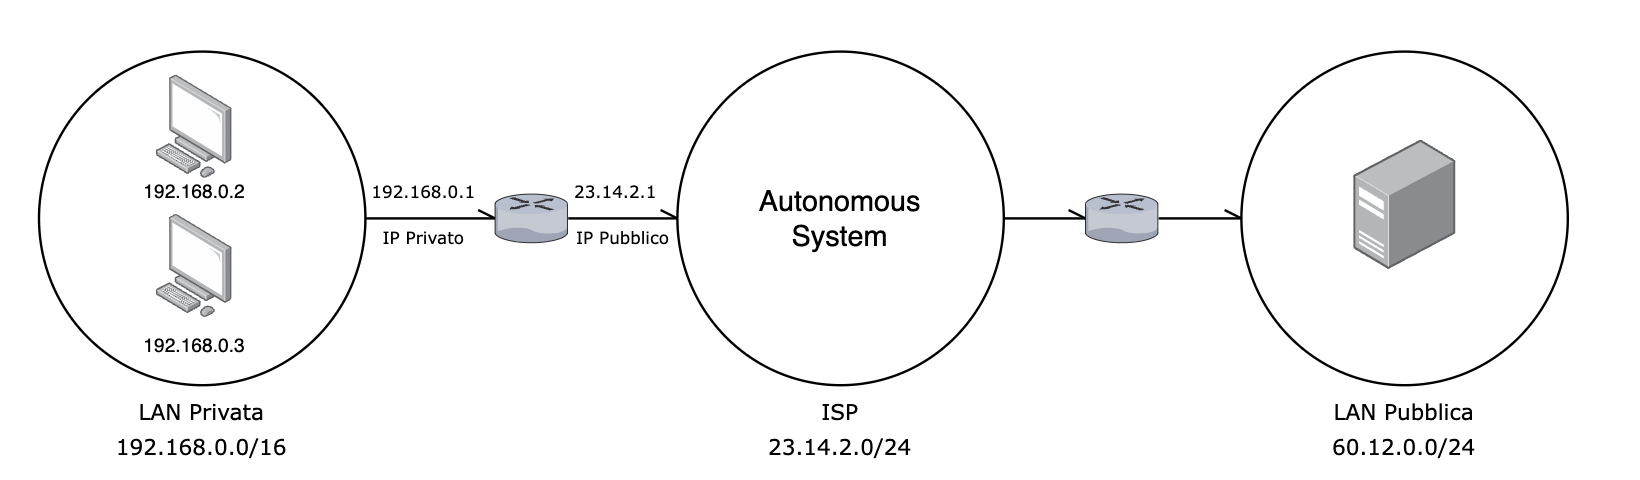
\includegraphics[width=1\textwidth]{NAT.png}
\end{figure}
\noindent
Il router (che possiede la funzionalità NAT) possiede due interfaccie, dove quella che punta verso la LAN privata ha un indirizzo privato e quella che punta all'esterno ha un indirizzo pubblico.
Dall'esterno, la nostra LAN privata sembrerà un unico host con un indirizzo IP pubblico.
È stato introdotto per sopperire alla scarsità degli indirizzi IP pubblici.
\begin{examplebox}{Domanda 3}
    In riferimento al livello di trasporto, si spieghi che cosa sono le “porte note” (Well Known Ports) e il
    motivo per cui sono state introdotte.
\end{examplebox}
\noindent
In generale, a livello di trasporto esistono delle porte note (Well Known Ports) che sono state introdotte per permettere la comunicazione tra i vari servizi offerti da un host.
Queste porte sono numerate da 0 a 1023 e sono riservate per i servizi più comuni, come ad esempio i protocolli HTTP, SMTP, utilizzati \textbf{lato server}.

\section{Esercizi}

\subsection{Esercizio Livello Data Link}

Un Bridge è attestato contemporaneamente su due segmenti distinti di
rete; sul segmento 1 c’è una stazione, A, e sul segmento 2 c’è una
stazione, B (si veda la figura a fianco). Il Bridge è un particolare tipo di
stazione che memorizza ciascuna trama che arriva da un segmento di
rete e, una volta ricevuta completamente, la ritrasmette sull’altro
segmento di rete (tale comportamento è valido, in modo indipendente
l’uno dall’altro, in entrambi i sensi); le trame restano in memoria del
Bridge fino a quando la trasmissione sull’altro segmento non è andata
a buon fine. Le stazioni e il Bridge utilizzano un protocollo ALOHA. Le caratteristiche del sistema sono:
\begin{itemize}
    \item $v_1 = 1.2$ Mbit/s
    \item $v_2 = 800$ Kbit/s
    \item $L = 1200$ byte
    \item $\tau_1 = \tau_2 = 0$
\end{itemize}
Le trame che vengono generate sono le seguenti:
\begin{itemize}
    \item $T_{A1} = 415$ ms diretta a $B$
    \item $T_{A2} = 435$ ms diretta a $B$
    \item $T_{B1} = 415$ ms diretta a $A$
    \item $T_{B2} = 430$ ms diretta a $A$
\end{itemize}
\begin{figure}[H]
    \centering
    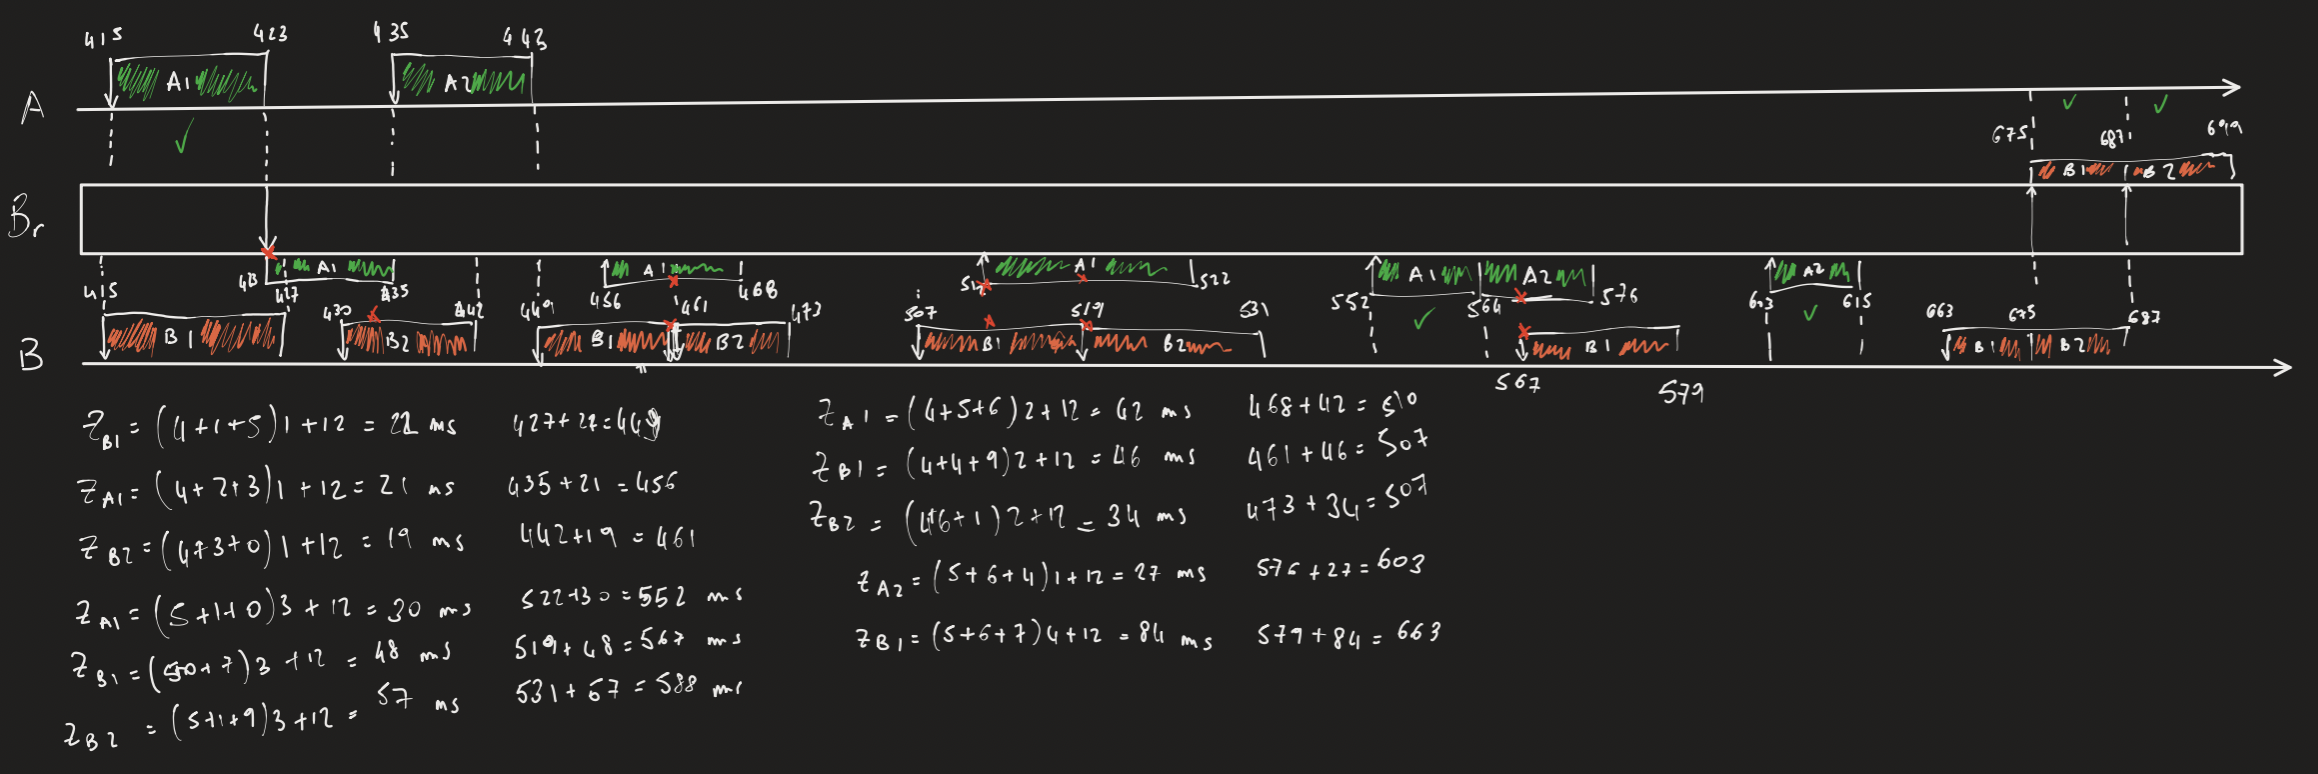
\includegraphics[width=1\textwidth]{ESDL1.png}
\end{figure}


\subsection{Esercizio Livello Trasporto}

Un’applicazione A deve trasferire 83200 byte all’applicazione B utilizzando il protocollo TCP. Si supponga che
la connessione tra A e B sia già stata instaurata. La trasmissione dei segmenti inizia al tempo t=0. Sono noti i
seguenti parametri:

\begin{itemize}
    \item MSS 1300 byte
    \item RCWND: 20800 byte. A partire da $t_a > 11$ la destinazione annuncia una RCWND pari a $15600$ byte
    \item STT = RCWND
    \item CWND=1 quando $t=0$
    \item RTT = 1s
    \item RTO = 2RTT
    \item Down di rete: [4 - 5] e [11.5 - 13]
\end{itemize}

\begin{figure}[H]
    \centering
    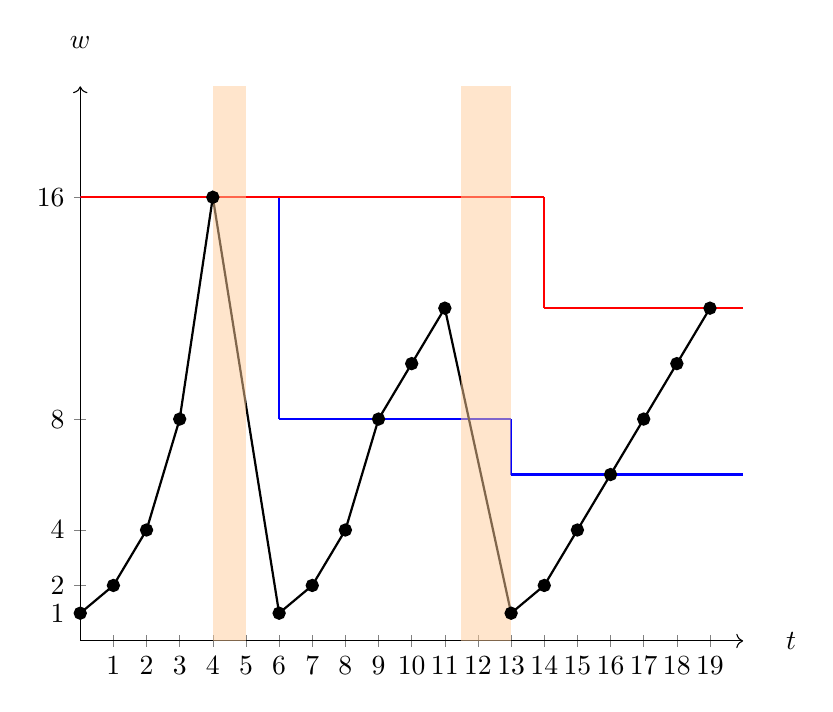
\begin{tikzpicture}
        \begin{axis}[
            axis lines=middle,
            xlabel={$t$},
            ylabel={$w$},
            xtick={0,1,2,3,4,5,6,7,8,9,10,11,12,13,14,15, 16, 17, 18, 19},
            ytick={1,2,4,8, 16},
            ymin=0, ymax=20,
            xmin=0, xmax=20,
            axis line style={->},
            every axis x label/.style={
                at={(ticklabel* cs:1.05)},
                anchor=west,
            },
            every axis y label/.style={
                at={(ticklabel* cs:1.05)},
                anchor=south,
            }
        ]
        
        % Draw the STT Threshold
        \addplot[domain=0:6, samples=100, color=blue, thick]{16};
        \addplot[color=blue, thick] coordinates {(6, 16) (6, 8)};
        \addplot[domain=6:13, samples=100, color=blue, thick]{8};
        \addplot[color=blue, thick] coordinates {(13, 8) (13, 6)};
        \addplot[domain=13:20, samples=100, color=blue, thick]{6};

        \addplot[domain=0:14, samples=100, color=red, thick]{16};
        \addplot[color=red, thick] coordinates {(14, 16) (14, 12)};
        \addplot[domain=14:20, samples=100, color=red, thick]{12};


        % Draw the plot and points
        \addplot[thick, mark=*] coordinates {(0, 1) (1,2) (2,4) (3,8) (4, 16) (6, 1) (7,2) (8,4) (9, 8) (10, 10) (11, 12) (13, 1) (14,2) (15, 4) (16, 6) (17, 8) (18, 10) (19, 12)} ;
        \fill[orange!40, opacity=0.5] (4, 0) rectangle (5, 20);
        \fill[orange!40, opacity=0.5] (11.5, 0) rectangle (13, 20);
        
        \end{axis}
      \end{tikzpicture}
    \end{figure}

    \[\# Seg = 1 + 2 + 4 + 8 + \cancel{16} + 1 + 2 + 4 + 8 + 10 + \cancel{12} + 1 + 2+ 4 + 6 + 8 + 3 = 64\]
    \[CWND_{finale} = CWND_{old} + \frac{\#ACK}{CWND_{old}} = 10 + \frac{3}{10}\]
    \[t_{fin} = 19\]
\subsection*{Esercizio Livello Rete}

Si consideri la rete rappresentata in Figura, collegata ad
Internet attraverso il router C (router di default per la
rete). Si hanno i seguenti vincoli:
\begin{itemize}
    \item la LAN 1 contiene un host con indirizzo
    76.104.213.12;
    \item Le LAN 1, 2, e 3 devono poter contenere
    rispettivamente almeno 300, 1200, e 520 host.
\end{itemize}
In base ai suddetti vincoli:
\begin{enumerate}
    \item Si specifichi il blocco CIDR più piccolo da assegnare alla rete;
    \item Si assegnino gli indirizzi di rete e di broadcast alle LAN 1, 2, e 3, utilizzando il blocco CIDR individuato
    nel punto precedente.
    \item Si scriva la tabella di routing del router A, considerando come metrica il numero di hop e assumendo
    che il router X abbia annunciato di poter raggiungere qualsiasi host su Internet in 4 hop.    
\end{enumerate}
\noindent
Blocco CIDR totale:
\[76. \; \; 104. \; \; \overbrace{\colorbox{blue!30!white}{1101}0000}^{208} \; \; \overbrace{00000000}^{0} \Longrightarrow 76.104.208.0/20\]
\textbf{LAN 2 \& Broadcast:} 
\[76. \; \; 104. \; \; \overbrace{\colorbox{blue!30!white}{1101}\colorbox{green!30!white}{1}000}^{216} \; \; \overbrace{00000000}^{0} \Longrightarrow 76.104.216.0/21\]
\[76. \; \; 104. \; \; \overbrace{\colorbox{blue!30!white}{1101}\colorbox{green!30!white}{1}111}^{216} \; \; \overbrace{11111111}^{255} \Longrightarrow 76.104.223.255/21\]
\textbf{LAN 3:}
\[76. \; \; 104. \; \; \overbrace{\colorbox{blue!30!white}{1101}\colorbox{green!30!white}{00}00}^{208} \; \; \overbrace{00000000}^{0} \Longrightarrow 76.104.208.0/22\]
\[76. \; \; 104. \; \; \overbrace{\colorbox{blue!30!white}{1101}\colorbox{green!30!white}{00}11}^{211} \; \; \overbrace{11111111}^{255} \Longrightarrow 76.104.211.255/22\]
\textbf{LAN 1:}
\[76. \; \; 104. \; \; \overbrace{\colorbox{blue!30!white}{1101}\colorbox{green!30!white}{010}0}^{212} \; \; \overbrace{00000000}^{0} \Longrightarrow 76.104.212.0/23\]
\[76. \; \; 104. \; \; \overbrace{\colorbox{blue!30!white}{1101}\colorbox{green!30!white}{010}1}^{213} \; \; \overbrace{11111111}^{255} \Longrightarrow 76.104.213.255/23\]

\noindent
La tabella di routing del ROUTER A:

\begin{table}[H]
    \centering
    \begin{tabular}{c|c|c}
        \textbf{Destinazione} & \textbf{Next Hop} & \textbf{Costo} \\ \hline
        LAN1 & diretto  & 1 \\
        LAN2 & B & 2 \\
        LAN3 & diretto &1\\
        Internet & C & 5 \\
    \end{tabular}
\end{table}

\end{document}
